\documentclass{article}
\setlength{\parindent}{0ex}
\setlength{\parskip}{1em}
\usepackage[utf8]{inputenc} 
\usepackage{amsfonts}
\usepackage{amsmath}
\usepackage{amsthm}
\renewenvironment{proof}[1][\proofname]{{\bfseries #1.}}{\qed}
\usepackage{amssymb}
\usepackage{amstext}
\usepackage{fancybox}
\usepackage{tikz}
\usepackage{tkz-euclide}
\usepackage{gensymb}
\usepackage{graphicx}
\usepackage{verbatim}
\usepackage{qtree}
\usepackage{scrextend}
\usepackage{multirow}
\usepackage{float}
\usepackage{algpseudocode}
\usepackage[bottom]{footmisc}
\usepackage[toc,page]{appendix}
\usepackage{pbox}


\tikzset{main node/.style={circle,fill=blue!20,draw,minimum size=1cm,inner sep=0pt},
}


%Kodestyling \begin{lstlisting}
\usepackage{color}
\usepackage{listings}
\lstset{ %
language=C++,                % choose the language of the code
%basicstyle=\footnotesize,       % the size of the fonts that are used for the code
basicstyle=\ttfamily,
numbers=left,                   % where to put the line-numbers
numberstyle=\footnotesize,      % the size of the fonts that are used for the line-numbers
stepnumber=1,                   % the step between two line-numbers. If it is 1 each line will be numbered
numbersep=5pt,                  % how far the line-numbers are from the code
backgroundcolor=\color{white},  % choose the background color. You must add \usepackage{color}
showspaces=false,               % show spaces adding particular underscores
showstringspaces=false,         % underline spaces within strings
showtabs=false,                 % show tabs within strings adding particular underscores
frame=single,           % adds a frame around the code
tabsize=2,          % sets default tabsize to 2 spaces
captionpos=b,           % sets the caption-position to bottom
breaklines=true,        % sets automatic line breaking
breakatwhitespace=false,    % sets if automatic breaks should only happen at whitespace
escapeinside={\%*}{*)},          % if you want to add a comment within your code
mathescape
}

\def\multiset#1#2{\ensuremath{\left(\kern-.3em\left(\genfrac{}{}{0pt}{}{#1}{#2}\right)\kern-.3em\right)}}

\usepackage{caption}

\usepackage{mathtools}
\DeclarePairedDelimiter\ceil{\lceil}{\rceil}
\DeclarePairedDelimiter\floor{\lfloor}{\rfloor}


\def\meta#1{\mbox{$\langle\hbox{#1}\rangle$}}
\def\macrowitharg#1#2{{\tt\string#1\bra\meta{#2}\ket}}

{\escapechar-1 \xdef\bra{\string\{}\xdef\ket{\string\}}}

\def\intro#1{{#1}{\cal I}}
\def\elim#1{{#1}{\cal E}}

\showboxbreadth 999
\showboxdepth 999
\tracingoutput 1


\let\imp\to
\def\elim#1{{{#1}{\cal E}}}
\def\intro#1{{{#1}{\cal I}}}
\def\lt{<}
\def\eqdef{=}
\def\eps{\mathrel{\epsilon}}
\def\biimplies{\leftrightarrow}
\def\flt#1{\mathrel{{#1}^\flat}}
\def\setof#1{{\left\{{#1}\right\}}}
\let\implies\to
\def\KK{{\mathsf K}}
\let\squashmuskip\relax

\graphicspath{ {images/} }
\usetikzlibrary{arrows}
\tikzset{
  leaf_/.style = {shape=rectangle,draw, align=center},
  node_/.style     = {shape=circle,draw,align=center}
}
\author{Rune Kok Nielsen (qkd362), Andreas Holm (jnh508)}
\title{GraphHopper kernel in C++}
\DeclareMathOperator{\Ran}{Ran}
\DeclareMathOperator{\Dom}{Dom}

\renewcommand*\contentsname{Contents}
\begin{document}
	
\maketitle
\newpage
\tableofcontents
\newpage

\section{Introduction}
This report presents our work and the theory used developing and testing an efficient implementation of the GraphHopper kernel in C++ for our Bachelor thesis. While we do introduce the basics behind SVM and kernels based on our earlier work in \cite{svm-graph-kernels} the focus will primarily lie on the algorithm behind the kernel itself as well as the introduction of \textit{Gaps}. After presenting the theory we will provide the results of our experiments analysing the time efficiency of our implementation compared to an existing MATLAB-implementation as well as the effect on classification accuracy in different datasets when adding \textit{Gaps} to the kernel. 

\section{SVM (Short summary)}
Before we start introducing graphhopper we want to give a short summary of some of the key concepts in the topic support vector machines (svm), in this summary we will primarily focus on the basic concepts of classification, svm, graph kernels and cross validation. This summary is based on our former report \cite{svm-graph-kernels}, which does a more thoroughly introduction to the topics.

\subsection{Classification}
The root problem and what we are trying to achieve with svm's is we want to try to solve the classification problem, the classification problem is that you are given an amount of records, where each record needs to be classified. To solve this problem we use a classification technique which is known as support vector machines.

\subsection{SVM}
Support vector machines (svm) is a binary classification technique which is used to predict classification of records in data, which consist of multiple dimensions. In figure \ref{fig:hyperplane} it is show how the svm will predict with a hyperplane which classification each of the nodes belong to, this example is based on linear svm, but we can also make a non-linear svm, when we are doing a non-linear svm it start to get complexed, because we still want to draw a linear hyperplane, and to do this we need to transform the data to a new dimension where these points can be split with a linear hyperplane. These transformations are unknown and can be hard to find, but with mercer's theorem it is show how we can use graph kernels to instead of transforming, see \cite{svm-graph-kernels} for a better description of mercer's theorem.
\begin{figure}[H]
	\centering
	\includegraphics[width=10cm]{svm_plot}
	\caption{\textit{aoeu}}
	\label{fig:hyperplane}
\end{figure}

\subsection{Graph kernel}
Mercer's theorem says that if we have a symmetrical and positive semi-definite function, then there exist a transformation.

In (\ref{eq:kernel_function}) is it shown how the kernel function is connected to the svm, as seen in the formula it is attached to the optimization problem know as the dual lagrange problem.
\begin{equation}
\label{eq:kernel_function}
L_D = \sum_{i=1}^{n}\lambda_i-\frac{1}{2}\sum_{i,j}\lambda_i\lambda_j y_iy_jk(x_i,x_j)
\end{equation}

\subsection{Cross validation}
Cross validation is a concept we use when test our graph kernels, the basic concepts of cross validation is that we train our svm on a certain amount of the data, and then use the last amount of data, that the svm has not seen yet, to test how well it performs.

\section{GraphHopper}
\label{section:graphhopper}
The following description of the GraphHopper kernel is based on the presentation in \cite{graphhopper}.

GraphHopper is a graph kernel, i.e. a kernel for comparing graph data. The kernel effectively analyses the structure of the graphs by comparing shortest paths similarly to \textit{shortest path kernel}\footnote{We introduce the shortest path kernel in our earlier work \cite{svm-graph-kernels}.} (SPK). An advantage of these kernels is that they may analyse the structure of the graphs along with the properties of their nodes.
While SPK compares all shortest paths with a complexity of $\mathcal{O}(n^4)$, where $n$ is the number of nodes, GraphHopper only compares shortest paths of equal length with complexity $\mathcal{O}(n^2(m+\log n+\delta^2 + d))$ where $m$ is the number of edges, $\delta$ is the diameter of the graph and $d$ is the dimension of the node attributes. The complexity will be explained along with the algorithm itself.

Let $G=(V,E)$ and $G'=(V',E')$ be graphs such that $V,V'$ are nodes and $E,E'$ are edges and let $P,P'$ be the sets of all shortest paths in $G$ and $G'$ respectively. The kernel is then a sum of path kernel $k_p$ over each pair of shortest paths $\pi\in P,\ \pi'\in P'$:

\begin{equation}
\label{eq:k}
k_{graphhopper}(G,G')=\sum_{\pi\in P}\sum_{\pi'\in P'}k_p(\pi, \pi')
\end{equation}
The path kernel $k_p$ is a sum of some node kernel $k_n$ on each pair of nodes $v\in\pi,\ v'\in\pi'$ such that $v$ and $v'$ appears at the same place in $\pi$ and $\pi'$ for pairs $\pi$ and $\pi'$ of equal discrete length\footnote{Discrete length meaning that $\pi$ and $\pi'$ contains the same number of nodes.}. I.e.
\begin{equation}
\label{eq:k_p}
k_p(\pi, \pi')=\begin{cases}
\sum_{i=1}^{|\pi|}k_n(\pi(i), \pi'(i)) & \text{for }|\pi|=|\pi'|\\
0 & \text{otherwise}
\end{cases}
\end{equation}
where $\pi(i)$ denotes the $i$'th node in $\pi$. The node kernels that we have chosen to implement are all described in a later section and are not essential in describing the kernel itself.

Using the definition above we now present a simple example. Consider the two graphs, $G$ and $G'$ in figure \ref{fig:shortest-path-graph}.


\begin{figure}[H]
	\begin{minipage}[t]{0.7\linewidth}
		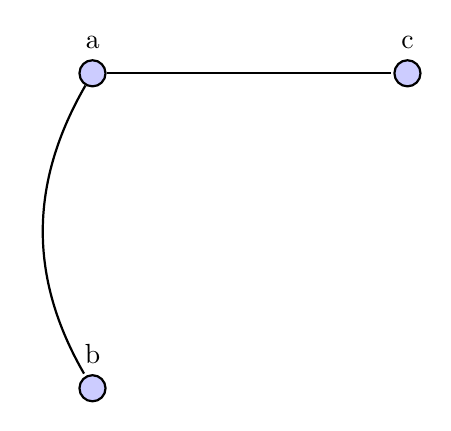
\begin{tikzpicture}[-,>=stealth',shorten >=1pt,auto,node distance=4cm,
		thick,main node/.style={circle,fill=blue!20,draw,font=\sffamily\Large\bfseries}]
		
		\node[main node] (a) [label=a] {};
		\node[main node] (b) [below of=a, label=b] {};
		\node[main node] (c) [right of=a, label=c] {};
		
		
		\path[every node/.style={font=\sffamily\small}]
		(a) edge [bend right] node {}(b)
		(a) edge node {}(c)
		;
		\end{tikzpicture}
	\end{minipage}
	\begin{minipage}[t]{0.2\linewidth}
		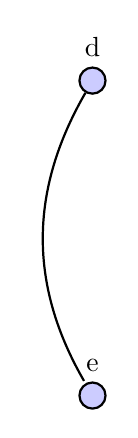
\begin{tikzpicture}[-,>=stealth',shorten >=1pt,auto,node distance=4cm,
		thick,main node/.style={circle,fill=blue!20,draw,font=\sffamily\Large\bfseries}]
		
		
		\node[main node] (d) [label=d] {};
		\node[main node] (e) [below of=d, label=e] {};
		
		
		\path[every node/.style={font=\sffamily\small}]
		(d) edge [bend right] node {}(e)
		;
		\end{tikzpicture}
	\end{minipage}
	\caption{\textit{Left: G. Right: G'}}
	\label{fig:shortest-path-graph}
\end{figure}
Identifying shortest paths we get
\begin{align*}
P&=\{[a], [a,b], [a,c], [b], [b,a], [b,a,c], [c], [c,a], [c,a,b]\}\\
P'&=\{[d],[d,e],[e],[e,d]\}
\end{align*}
We can now compute $k_{graphhopper}$ by summing over all paths $\pi\in P$ and $\pi'\in P'$ such that $|\pi|=|\pi'|$. E.g. the pair $\pi=[a]\in P,\ \pi'=[d]\in P'$ are of equal discrete length so we add $k_n(a, d)$ to the sum. Identifying more pairs we find, for instance, that $|\pi|=|\pi'|$ for $\pi=[a,b]\in P,\ \pi'=[d,e]\in P'$ so we add $k_n(a,d) + k_n(b, e)$. For completeness of the example the entire sum can be seen in (\ref{eq:example_sum}).

\begin{equation}
\label{eq:example_sum}
\begin{split}
k_{graphhopper}(G,G')	&=  \underbrace{k_n(a,d)}_{k_p([a],[d])} + \underbrace{k_n(a, e)}_{k_p([a],[e])} + \underbrace{k_n(a, d) + k_n(b, e)}_{k_p([a,b],[d,e])} + \underbrace{k_n(a, e) + k_n(b, d)}_{k_p([a,b],[e,d])} \\ 
				&+ \underbrace{k_n(a, d) + k_n(c, e)}_{k_p([a,c],[d,e])} + \underbrace{k_n(a, e) + k_n(c, d)}_{k_p([a,c],[e,d])} + \underbrace{k_n(b, d)}_{k_p([b],[d])} + \underbrace{k_n(b, e)}_{k_p([b],[e])} \\
				&+ \underbrace{k_n(b, d) + k_n(a, e)}_{k_p([b,a],[d,e])} + \underbrace{k_n(b, e) + k_n(a, d)}_{k_p([b,a],[e,d])} + \underbrace{k_n(c, d)}_{k_p([c],[d])} + \underbrace{k_n(c, e)}_{k_p([c],[e])} \\
				&+ \underbrace{k_n(c, e) + k_n(a, d)}_{k_p([c,a],[d,e])}+ \underbrace{k_n(c, d) + k_n(a, e)}_{k_p([c,a],[e,d])}
\end{split}
\end{equation}

Observe how we added $k_n(a,d)$ multiple times to the final sum. Naturally, the number of times $k_n(v, v')$ will be added (where $v\in V,\ v'\in V'$) will be exactly the number of pairs of paths $\pi\in P,\ \pi'\in P'$ such that $|\pi|=|\pi'|$ and $\pi(i)=v,\ \pi'(i)=v'$ for some $i$.

Let $w(v, v')$ be the number of times we have to add $k_n(v, v')$ for some pair $v\in V,\ v'\in V'$ as described above. Instead of computing and adding $k_n(v, v')$ repeatedly we may instead add $w(v,v') k_n(v, v')$ once. We call $w(v, v')$ the $\textit{weight}$ between the two nodes and rewrite the kernel as a weighted sum between pairs of nodes:
\begin{equation}
\label{eq:k_graphhopper}
k_{graphhopper}(G,G')=\sum_{v\in V}\sum_{v'\in V'}w(v,v')k_n(v,v')
\end{equation}


When calculating $w(v,v')$ we sum the number of pairs $\pi,\pi'$ such that $|\pi|=|\pi'|$ and $\pi(i)=\pi'(i)$ for some $i$. Let $width(G)$ be the discrete length of the longest shortest path $\pi\in P$ and let $\delta=min(width(G), width(G'))$. Since we only consider pairs of paths of same length and the longest shortest path we do not have to consider any paths of length greater than $\delta$.

\iffalse
\begin{proof}[Proof: We may ignore paths of length greather than $\delta$]\\
Consider any two graphs $G,\ G'$ such that $width(G)=\delta$. Then we either have $\delta=width(G')$ or $\delta<width(G')$.\\
Let $width(G)=\delta=width(G')$ and let $\pi'\in P'$ such that $|\pi'|>\delta$. Since $G'$ is at least as wide as any shortest paths within it we have $width(G')\geq |\pi'|>\delta = width(G')$ which is an absurdity.\\
Let $width(G)=\delta < width(G')$ and let $\pi'\in P'$ such that $|\pi'|>\delta$. Now assume that there exists some $\pi\in P$ such that $|\pi|=|\pi'|$. We now see that $width(G)\geq |\pi| = |\pi'|>\delta=width(G)$ which is an absurdity.\\
We have now proven that there can not exist any pairs of paths $\pi\in P,\ \pi'\in P'$ such that $|\pi|=|\pi'|>\delta$.
\end{proof}
\fi

Beside from this limitation it is trivial that for a pair of paths $\pi,\ \pi'$ such that $|\pi|=|\pi'|=j$ we only have to consider nodes at index $i=1..j$ since there cannot exist any nodes at index $i>j$.


We can now formalize $w(v,v')$ as
\begin{equation}
w(v,v')=\sum_{j=1}^{\delta}\sum_{i=1}^{j}|\{(\pi, \pi')\ |\ \pi(i)=v,\ \pi'(i)=v',\ |\pi|=|\pi'|=j\}|
\end{equation}


Let $\delta=width(G)$ and let $M$ be a $|V|\times\delta\times\delta$ matrix such that $M(v)_{ij}$ is the number of shortest paths $\pi\in P$ such that $|\pi|=j$ and $\pi(i)=v$. We then have
\begin{equation}
w(v,v')=\sum_{j=1}^{\delta}\sum_{i=1}^{j}M(v)_{ij}*M'(v')_{ij}
\label{eq:wmm}
\end{equation}
allowing us to easily find the weight between pairs of nodes by first computing $M$ and $M'$. Furthermore, when computing $K$ for multiple graphs we may compute all M matrices beforehand and use them in the pairwise computations instead of computing them for each pair of graphs.


\subsection{Computing $M$}
The $M$ matrix can be computed in a number of ways. We will be using the message-passing algorithms presented in \cite{graphhopper}

Let $\tilde{v}$ be a node in $V$ and let $P_{\tilde{v}}$ be the set of shortest paths in $G$ starting in $\tilde{v}$. Then $M(v)_{ij}$ becomes $\sum_{\tilde{v}\in V}$ number of times $v$ appears as the $i$'th node in each $\pi_{\tilde{v}}\in P_{\tilde{v}}$ of discrete length $j$. This means that we can compute $M$ by iterating over each node $\tilde{v}\in V$ and finding all shortest paths starting in $\tilde{v}$.

Before we move on, we will first introduce the shortest path DAG $G_{\tilde{v}}=(V, E_{\tilde{v}})$ for $\tilde{v}$ where $E_{\tilde{v}}$ are edges kept in $G_{\tilde{v}}$. The shortest path DAG $G_{\tilde{v}}$ is created by removing a minimum amount of edges from $G$ so that it only contains edges that are part of some shortest path starting in $\tilde{v}$. We call $\tilde{v}$ the root node in the resulting DAG. This is illustrated in figure \ref{fig:shortest-path-dag} where we present a graph $G$ and the shortest path DAG $G_{a}$ rooted in $a$.

\begin{figure}[H]
	\begin{minipage}[t]{0.7\linewidth}
		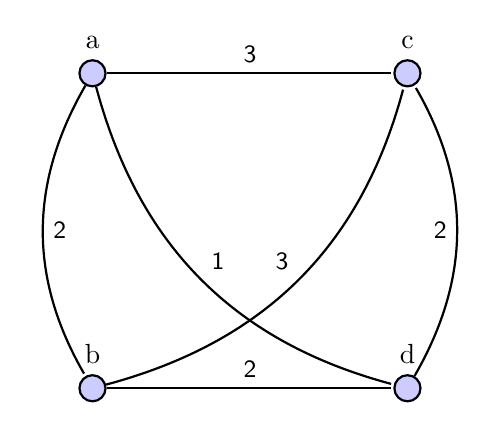
\begin{tikzpicture}[-,>=stealth',shorten >=1pt,auto,node distance=4cm,
		thick,main node/.style={circle,fill=blue!20,draw,font=\sffamily\Large\bfseries}]
		
		\node[main node] (a) [label=a] {};
		\node[main node] (b) [below of=a, label=b] {};
		\node[main node] (c) [right of=a, label=c] {};
		\node[main node] (d) [below of=c, label=d] {};
		
		
		\path[every node/.style={font=\sffamily\small}]
		(a) edge [bend right] node {2}(b)
		(a) edge node {3}(c)
		(a) edge [bend right] node {1}(d)
		(d) edge [bend right] node {2}(c)
		(b) edge node {2}(d)
		(b) edge [bend right] node {3}(c)
		;
		\end{tikzpicture}
	\end{minipage}
	\begin{minipage}[t]{0.2\linewidth}
		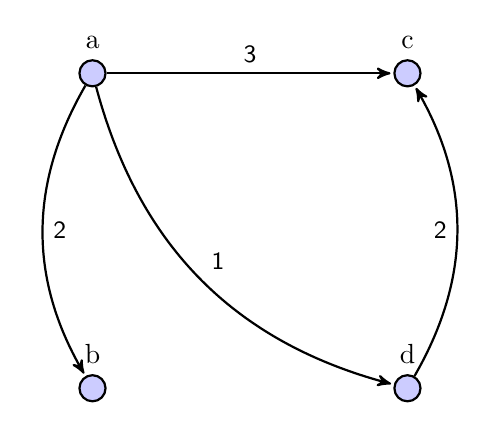
\begin{tikzpicture}[->,>=stealth',shorten >=1pt,auto,node distance=4cm,
		thick,main node/.style={circle,fill=blue!20,draw,font=\sffamily\Large\bfseries}]
		
		
		\node[main node] (a) [label=a] {};
		\node[main node] (b) [below of=a, label=b] {};
		\node[main node] (c) [right of=a, label=c] {};
		\node[main node] (d) [below of=c, label=d] {};
		
		
		\path[every node/.style={font=\sffamily\small}]
		(a) edge [bend right] node {2}(b)
		(a) edge node {3}(c)
		(a) edge [bend right] node {1}(d)
		(d) edge [bend right] node {2}(c)
		;
		\end{tikzpicture}
	\end{minipage}
	\caption{\textit{Left: G. Right: $G_{\tilde{a}}$}}
	\label{fig:shortest-path-dag}
\end{figure}

We now introduce two more constructs used for computing $M$: $\mathfrak{O}_{\tilde{v}}$ and $\mathfrak{D}_{\tilde{v}}$. 

\subsubsection{Computing $\mathfrak{O}_{\tilde{v}}$}
Let $\mathfrak{O}_{\tilde{v}}$ be a $n\times\delta$ matrix where $\mathfrak{O}_{\tilde{v}}(v,i)$ is the number of paths from $\tilde{v}$ to $v$ in the shortest path DAG $G_{\tilde{v}}$ with discrete length $i$.

\textbf{Example}\\
Using the graph illustrated in figure \ref{fig:shortest-path-dag}, we find that there are two paths from $a$ to $c$ in $G_{\tilde{a}}$ of discrete length 2 and 3 so $\mathfrak{O}_{a}(c,1)=0,\ \mathfrak{O}_{a}(c,2)=1,\ \mathfrak{O}_{a}(c,3)=1$.

The rows of $\mathfrak{O}_{\tilde{v}}$, denoted by $\mathfrak{o}_{\tilde{v}}^v$, are computed recursively using a message-passing algorithm starting at the root. Intuitively, there is always exactly one path from the root to itself in the shortest path DAG and this path is of discrete length 1 so $\mathfrak{o}_{\tilde{v}}^{\tilde{v}}=[1]$. From the current node, the algorithm passes a message to each of its reachable neighbours (children) containing its own row shifted one place to the right and adds the contents to the child's row. The algorithm then repeats on the next level of nodes. This is illustrated in figure \ref{fig:compute_o}.


\begin{figure}[H]
	\includegraphics[width=12cm]{compute_o}
	\caption{\textit{Computing $\mathfrak{O}_{\tilde{a}}$ using message-passing. Detailed in appendix \ref{appendix:illustrations_compute_o}.}}
	\label{fig:compute_o}
\end{figure}


Before defining the algorithm for computing $\mathfrak{O}_{\tilde{v}}$ we must define two constructs. First, let $\oplus$ be left-aligned addition between two vectors such that their length is aligned. I.e.:
\begin{equation}
[a, b] \oplus [c, d, e] = [a + c, b + d, e]
\end{equation}
Now, let $V_{\tilde{v}}^j$ be the nodes in $G_{\tilde{v}}$ such that there exists some path from the root to $v$ in $G_{\tilde{v}}$ with discrete length $j$. The algorithm is shown in figure \ref{algorithm:o}.

\begin{figure}[H]
\begin{lstlisting}
$\mathfrak{o}_{\tilde{v}}^{\tilde{v}}=[1]$
$\mathfrak{o}_{\tilde{v}}^v=[0], for\ v\in V \ {\tilde{v}}$
for $j=1..\delta$
   for $v\in V_{\tilde{V}}^j$
      for $w$ in $v$.children
         $\mathfrak{o}_{\tilde{v}}^w=\mathfrak{o}_{\tilde{v}}^w\oplus[0,\mathfrak{o}_{\tilde{v}}^v]$
      end
   end
end
\end{lstlisting}
\caption{Algorithm for computing $\mathfrak{O}_{\tilde{v}}$}
\label{algorithm:o}
\end{figure}

When computing $\mathfrak{O}_{\tilde{v}}$ each node sends exactly one message of size $\leq \delta$ to all of its children which are then updated. I.e. $|E_{\tilde{v}}|$ messages of size $\leq \delta$ giving a complexity of $\mathcal{O}(|E_{\tilde{v}}|\delta) \leq \mathcal{O}(|E|\delta)$.

\subsubsection{Computing $\mathfrak{D}_{\tilde{v}}$}

Let $\mathfrak{D}_{\tilde{v}}$ be a $n\times\delta$ matrix where $\mathfrak{D}_{\tilde{v}}(v, i)$ is the number of paths of discrete length $i$ in $G_{\tilde{v}}$ starting in $v$.

\textbf{Example}\\
Consider the node $d$ in figure \ref{fig:shortest-path-dag}. From this node there is one path in $G_{\tilde{a}}$ to itself of discrete length 1 ($\pi_1=[d]$) and one path to $c$ of discrete length 2 ($\pi_2=[d,c]$) so $\mathfrak{D}_a(d,1)=1,\ \mathfrak{D}_a(d,2)=1,\ \mathfrak{D}_a(d,i)=0$ for $i\notin\{1,2\}$.

The algorithm for computing $\mathfrak{D}_{\tilde{v}}$ will, like in the case of $\mathfrak{O}_{\tilde{v}}$, be using a message-passing approach. In this case the row for node $v$ in $\mathfrak{D}_{\tilde{v}}$ is denoted by $\mathfrak{d}_{\tilde{v}}^v$. We start by observing that all nodes must have exactly one path of discrete length 1 (the path to themselves) so we initialize $\mathfrak{d}_{\tilde{v}}^v=[1],\ \forall v\in V$. The $\mathfrak{d}_{\tilde{v}}^v$ row for $v$ is then computed by adding (using the $\oplus$ operation defined earlier) the rows of its children shifted one place to the right. The rows of the children are computed recursively until a leaf node is reached and the result is then send up through the stack of recursive calls. This is illustrated in figure \ref{fig:compute_d}.
\begin{figure}[H]
	\includegraphics[width=12cm]{compute_d}
	\caption{\textit{Computing $\mathfrak{d}_{\tilde{a}}$ using message-passing.  Detailed in appendix \ref{appendix:illustrations_compute_d}.}}
	\label{fig:compute_d}
\end{figure}

A recursive algorithm for computing $\mathfrak{D}_{\tilde{v}}$ can then be written out as in figure \ref{algorithm:d}.

\begin{figure}[H]
\begin{lstlisting}
function compute_d_rec(v)
   if not $\mathfrak{d}_{\tilde{v}}^v$.is_computed
      for $w$ in $v$.children
         $\mathfrak{d}_{\tilde{v}}^v = \mathfrak{d}_{\tilde{v}}^v \oplus $[0,compute_d_rec(w)]
      end
      $\mathfrak{d}_{\tilde{v}}^v$.is_computed = true
   end
   return $\mathfrak{d}_{\tilde{v}}^v$
end
	
initialize: $\mathfrak{d}_{\tilde{v}}^v=[1],\ \forall v\in V$
compute_d_rec($\tilde{v}$)
	
\end{lstlisting}
	\caption{Algorithm for computing $\mathfrak{D}_{\tilde{v}}$}
	\label{algorithm:d}
\end{figure}

When computing $\mathfrak{D}_{\tilde{v}}$ with the algorithm detailed in figure \ref{algorithm:d} a node visits each of its children in $G_{\tilde{v}}$ exactly once when computing its row and in this process their rows are computed recursively. Effectively, each edge $e\in E_{\tilde{v}}$ will be traversed once and each time a message will be returned of size $\leq \delta$ which updates the calling node. This gives a complexity of $\mathcal{O}(|E_{\tilde{v}}|\delta)\leq(|E|\delta)$


\subsubsection{Putting things together}
Having computed $\mathfrak{O}_{\tilde{v}}$ and $\mathfrak{D}_{\tilde{v}}$ we now observe that the number of times that $v$ appears as the $i$'th node in a path of discrete length $j$ in $G_{\tilde{v}}$ must be the number of paths from $\tilde{v}$ to $v$ in $G_{\tilde{v}}$ of length $i$ times the number of paths of length $j-i+1$ in $G_{\tilde{v}}$ starting in $v$; i.e. $\mathfrak{O}_{\tilde{v}}^v(v,i)\mathfrak{D}_{\tilde{v}}(v,j - i + 1)$.

\textbf{Example}\\
Consider the node $d$ in figure \ref{fig:shortest-path-dag}. Trying to find the number of paths in $G_{a}$ such that $d$ is the 2nd node in a path of length 3 we can intuitively see that there is one such path: $[a,d,c]$. This equivalent to the number of paths of length 2 from $a$ to $d$ times the number of paths of length $3-2+1=2$ starting in $d$.
This could be computed using the $\mathfrak{o}_a^d$ and $\mathfrak{d}_a^d$ computed earlier in figures \ref{fig:compute_o} and \ref{fig:compute_d}:
\begin{align}
\mathfrak{o}_a^d(2)\mathfrak{d}_a^d(3-2+1)&=\mathfrak{o}_a^d(2)\mathfrak{d}_a^d(2)\\
&=1 * 1\\
&=1
\end{align}

Being able to efficiently count the number of times $v$ appears as the $i$'th node in a path of length $j$ in a shortest path from $\tilde{v}$ we can now look back at the definition of $M(v)$ and conclude that

\begin{equation}
M(v)_{ij} = \sum_{\tilde{v}\in V}\mathfrak{o}_{\tilde{v}}^v(i)\mathfrak{d}_{\tilde{v}}^v(j-i+1)
\label{eq:runtime_comp_m}
\end{equation}

Computing $M$ may be achieved using the algorithm shown in figure \ref{alg:compute_M}. First we compute $G_{\tilde{v}},\mathfrak{O}_{\tilde{v}},\mathfrak{D}_{\tilde{v}}$ for all $\tilde{v}\in V$. Using a Dijkstra implementation\footnote{Using a binary-heap implementation as described in \cite{alg-bible} and assuming that all nodes are reachable.} with complexity $\mathcal{O}(m\log n)$ to compute $G_{\tilde{v}}$ this gives a complexity of $\mathcal{O}(n((m\log n) + m\delta + m\delta)) = \mathcal{O}(n((m\log n + m\delta))$. We then iterate over each pair of $v,\tilde{v}$ and $j=1..\delta,i=1..j$ giving a complexity of $\mathcal{O}(n^2\delta^2)$. Adding this together we get a total complexity of
\begin{align}
\mathcal{O}(n(m\log n + m\delta) + n^2\delta^2)&=\mathcal{O}(n(m\log n + m\delta + n\delta^2))
\end{align}

\begin{figure}[H]
\begin{lstlisting}
for $\tilde{v}\in V$
   compute $G_{\tilde{v}}$ using Dijkstra
   compute $\mathfrak{O}_{\tilde{v}}$
   compute $\mathfrak{D}_{\tilde{v}}$
end
let $M$ be a $n\times \delta \times \delta$ matrix of zeros
for $v \in V$
   for $\tilde{v}\in V$ 
      for $j\in 1..\delta$
         for $i\in 1..j$
            $M(v)_{ij}+=\mathfrak{o}_{\tilde{v}}^v(i)\mathfrak{d}_{\tilde{v}}^v(j-i+1)$
         end
      end
   end
end
\end{lstlisting}
\caption{Algorithm for computing M.}
\label{alg:compute_M}
\end{figure}

\subsection{Computational analysis}
To compute $k_{graphopper}$ we sum over each pair of nodes which, given precomputed $w(v,v')$ and $k_n(v,v')$, gives a complexity of $\mathcal{O}(n^2)$. Assuming that the complexity of computing $k_n(v,v')$ grows linearly relative to the dimension $d$ of the node attributes the complexity of computing all $k_n(v,v')$ has a complexity of $\mathcal{O}(n^2d)$. Computing the weight $w(v,v')$ between two nodes $v,v'$ (equation (\ref{eq:wmm})) consists of summing for $j\leq \delta,i\leq j$ giving $\mathcal{O}(\delta^2)$ and doing this for each pair gives a complexity of $\mathcal{O}(n^2\delta^2)$. Together this gives a complexity of $\mathcal{O}(n^2(d + \delta^2))$. Before doing these computations, however, we must first compute the $M$ matrices as described earlier (equation (\ref{eq:runtime_comp_m})) adding up to a total complexity of
\begin{align}
&\mathcal{O}\left(n^2\left(d + \delta^2\right) + n\left(m\log n + m\delta + n\delta^2\right)\right)\\
=\ &\mathcal{O}\left(n^2\left(d+\delta^2\right)+nm\left(\log n + \delta\right)\right)
\label{eq:k_one_pair}
\end{align}
for comparing two graphs where $n$ is the greatest number of nodes in a single graph, $m$ is the greatest number of edges in a single graph and $\delta$ is the greatest width of any graph. Typically we will not just be comparing two graphs. On the contrary, we will want to compute the inner product between all pairs of a large number of graphs. When doing so we can run the pairwise comparison more efficiently than described in (\ref{eq:k_one_pair}) as we may precompute all $M$ matrices before running the pairwise computations. Let $N$ be the number of graphs to compare. Then we must compute $N$ individual $M$ matrices. Using the complexity described in (\ref{eq:runtime_comp_m}) this gives a complexity of
\begin{equation}
\mathcal{O}\left(N\left(n\left(m\log n + m\delta + n\delta^2\right)\right)\right)
\end{equation}

We now have to compute $k_{graphhopper}$ on each unique pair of graphs. In practice, since a kernel is by definition symmetric, we do not consider all $N^2$ sequences. Instead, we count the number of multisets of cardinality 2 in the set of $N$ graphs, i.e. $\multiset{N}{2}$. This gives a complexity of
\begin{equation}
\mathcal{O}\left(\multiset{N}{2}\left(n^2\left(d+\delta^2\right)\right)\right)
\end{equation}
Adding the complexity of precomputing the $M$ matrices we land at a total complexity of
\begin{equation}
\mathcal{O}\left(\multiset{N}{2}\left(n^2\left(d+\delta^2\right)\right) + N\left(n\left(m\log n + m\delta + n\delta^2\right)\right)\right)
\end{equation}


\subsection{Implementation}
In this section we present the algorithm used in our implementation of GraphHopper described using pseudo-code. Based on the theory explained earlier we are able to effectively split the computation into two steps:
\begin{enumerate}
	\item Compute $M$ for all graphs.
	\item Compute $K$ using all pairs of M.
\end{enumerate}
The code presented here will not be a 1:1 match with the actual implementation but rather an introduction to the algorithm. We will exclude unneeded details including optimizations that are not required to understand the implementation.

\subsubsection{Computing M}

\begin{lstlisting}
#Computes the M matrix for a graph
function computeM($graph$){
   for $\tilde{v}\in graph.V$
      prepareNode($\tilde{v}$)
   end
   
   #Let M be an $|V|\times\delta\times\delta$ array of zeros
   $graph.M$ = array$[|graph.V|][graph.\delta][graph.\delta]$
   #Now sum the data of $\mathfrak{D}$ and $\mathfrak{O}$
   for $v\in graph.V$
      for $\tilde{v}\in graph.V$
         for $j\in 1..graph.\delta$
            for $i\in 1..j$
               $M[v][i][j] += \mathfrak{o}_{\tilde{v}}^v(i)\mathfrak{d}_{\tilde{v}}^v(j-i+1)$
            end
         end
      end
   end
}

#Computes $\mathfrak{O}_{\tilde{v}}$ and $\mathfrak{D}_{\tilde{v}}$
#Starts by creating $G_{\tilde{v}}$ using Dijkstra 
#before computing the matrices.
function prepareNode($graph$, $\tilde{v}$)
   #Prepare data for Dijkstra
   $queue = []$
   for $v\in graph.V$
      $v.d = \infty$
      $v.parents = []$
      $v.children = []$
      $queue.append(v)$
   end
   $\tilde{v}.d = 0$
   #$queue$ is a min heap allowing us to pop
   #the node with lowest d
   $queue.make\_min\_heap()$
   $\delta = 0$
   while not $queue.empty()$
      $u = queue.front()$
      $queue.pop()$
      
      $d = u.d + 1$
      for $v \in u.adjacent$
         if $v.d \geq d$
            if $v.d > d$
               $v.parents = []$
            end
            $v.parents.append(u)$
            $v.d = d$
            $\delta=max(\delta, d)$
         end
      end
      $queue.make\_min\_heap()$
   end
   #Set the graph's width to be the maximum width
   #found computing Dijkstra for any $\tilde{v}$
   $graph.\delta = max(graph.\delta, \delta)$
   
   #Putting nodes in buckets grouped and ordered
   #by shortest distance to $\tilde{v}$
   $\tilde{v}.ordered = $group_nodes($graph.V$)
   
   #Use $parents$ data to define $children$ in nodes
   prepare_children($graph.V$)
   
   #Refer to algorithms in last theory section
   computeO($\tilde{v},\ \delta$)
   computeD($\tilde{v}$)
end


\end{lstlisting}

\subsection{Gaps}
The following section is based on the description of GraphHopper with gaps on trees from \cite{gappy}. While this paper only describes the use of gaps on trees we will be expanding the definitions to also work on graphs in general.

Some of the graphs we wish to classify are extracted from images. Since the process of extraction is not perfect the resulting graphs may contain errors namely in form of missing edges. To minimize the impact of these error we can choose to allow gaps when comparing shortest paths. Allowing gaps allows us to create new paths called \textit{gappy paths} in the graphs which may skip up to $s$ nodes at a time (i.e. gaps of size $\leq s$). This may close some of the gaps where edges were missing. In figure \ref{fig:simple_gaps} is it shown how we can apply gaps to a simple graph.
\begin{figure}[H]
	\centering
	\includegraphics[width=12cm]{gaps}
	\caption{\textit{Left: No gaps. Middle: Gap size 1. Right: Gaps size 2.}}
	\label{fig:simple_gaps}
\end{figure}

Gappy paths are added to the shortest path DAG $G_{\tilde{v}}$ before computing $\mathfrak{O}_{\tilde{v}}$ and $\mathfrak{D}_{\tilde{v}}$. To add gappy paths we look at each pair of nodes $v,v'\in E_{\tilde{v}}$. We then add an edge $(v,v')$ to an updated set of edges $E'_{\tilde{v}}$ iff there exists a path in $G_{\tilde{v}}$ from $v$ to $v'$ of discrete length $\leq s + 2$. E.g. if there exists a path $\pi=[v_1,v_2,v_3]$ in $G_{\tilde{v}}$ and we allow gaps of size $s=1$ then the discrete length $|\pi| = 3 \leq s + 2 = 3$ so we add the edge $(v_1,v_2)$ to $E'_{\tilde{v}}$. This can be formalized as
\begin{equation}
\label{eq:gaps}
E'_{\tilde{v}} = E_{\tilde{v}} \cup \{ \forall(v, v')|\pi \in P_{G_{\tilde{v}}} \land \pi = [v,...,v'] \land |\pi| \leq s + 2 \}
\end{equation}

where $P_{G_{\tilde{v}}}$ is the set of all paths in $G_{\tilde{v}}$.

Adding gappy paths simply consists of adding new edges to the shortet path DAG. Afterwards we compute $M$ and eventually $K$ in the same way as we normally would as discussed in section \ref{section:graphhopper}.


\subsubsection{Implementation}
In this section we will show how simple it is to add gaps to our current graphhopper implementation.
\begin{lstlisting}
function prepareNode($graph$, $\tilde{v}$)

#Dijkstra completed

  if $s > 0$
    for $v \in graph.V$
      #Find all the new parents, 
      #with a gap of size $1$..$s$.
      $current\_parents = []$
      $tmp\_parents = v.parents$
      for $i \in 1..s$
        $current\_parents = tmp\_parents$
        $tmp\_parents.clear()$
        for $j \in 1..current\_parents.size()$
          for $k \in 1..current\_parents[j].parents.size()$
            $v.grandParents.append(current\_parents[j].parents[k])$
            $tmp\_parents.append(current\_parents[j].parents[k])$
          end
        end
      end

      #Find all the new children, 
      #with a gap of size $1$..$s$.
      $current\_children = []$
      $tmp\_children = v.parents$
      for $i \in 1..s$
        $current\_children = tmp\_children$
        $tmp\_children.clear()$
        for $j \in 1..current\_children.size()$
          for $k \in 1..current\_children[j].children.size()$
            $v.grandChildren.append(current\_children[j].children[k])$
            $tmp\_children.append(current\_children[j].children[k])$
          end
        end
      end
    end
  end

  #Move grandparents/grandchildren
  #to parents/children.
  for $v \in graph.V$
    while not $v.grandParents.empty()$
      $v.parents.append(v.grandParents.pop())$
    end
    while not $v.grandChildren.empty()$
      $v.children.append(v.grandChildren.pop())$
    end
  end

  #After adding the new paths, we can call:
  #computeO and computeD

end
\end{lstlisting}

\section{Node kernels}
As mentioned in section $\ref{section:graphhopper}$ one of the advantages of GraphHopper is that we apply any node kernel to compare the nodes. In this section we introduce the node kernels that we have chosen to include in our implementation. The following equations will be comparing two values $x,x'$ which when used as node kernel represent the labels of two nodes $v,v'$.

\subsection{Dirac}
Dirac is a simple kernel best suited for comparing discrete values representing non-continuous data, e.g. class labels. The kernel returns 1 if the two values are equal and 0 otherwise. The kernel is formally described in (\ref{eq:dirac}).
\begin{equation}
\label{eq:dirac}
k_{dirac}(x, x')=\begin{cases}
1 & \text{for }x=x'\\
0 & \text{otherwise}
\end{cases}
\end{equation}

\subsection{Linear}
The linear node kernel is the dot product of $x$ and $x'$ as formally described in (\ref{eq:linear}).
\begin{equation}
\label{eq:linear}
k_{linear}(x, x') = x(i) \cdot x'(i)
\end{equation}

\subsection{Gaussian}
The Gaussian kernel is a popular choice for comparing continuous data. The kernel is formally defined in equation (\ref{eq:gaussian}). When two values are equal to each other the kernel returns 1 and the more they differ the closer the result gets to 0. By fine tuning the $\sigma$ parameter (e.g. by cross-validation) you may achieve a smooth curve that manages to describe the similarity of two values in a non-binary way by assigning a value between 0 and 1.

\begin{equation}
\label{eq:gaussian}
k_{gaussian}(x, x') = exp(-\frac{||x - x'||^2}{2\sigma^2})
\end{equation}

Our implementation is based on an optimized equation as defined in (\ref{eq:gaussian_simple}) where $\mu=\frac{1}{2\sigma^2}$. The two equations yield the same result but using $\mu$ as a parameter instead of $\sigma$ we save time by eliminating some calculations.

\begin{equation}
\label{eq:gaussian_simple}
k_{gaussian}(x, x') = exp(-\mu ||x - x'||^2)
\end{equation}

The curve of the Gaussian kernel is illustrated in figure \ref{fig:gaussian_graph} where the $x$ axis represents the difference between two values and the $y$ axis represents the result yielded by this Gaussian funciton. The width of the curve is controlled by the $\sigma$ parameter. When $\sigma$ grows the curve gets wider and as such the function allows for more dissimilarity.

\begin{figure}[H]
	\centering
	\includegraphics[width=10cm]{gaussian}
	\caption{\textit{Illustration of the Gaussian kernel for $\sigma = 0.3$}}
	\label{fig:gaussian_graph}
\end{figure}


\subsection{Bridge}
The Bridge kernel\footnote{As defined in \cite{shortest-path}} as formalized in equation (\ref{eq:bridge}) is similar to the Gaussian kernel in that it yields a result between 0 (for very dissimilar values) and some constant $c>0$ for equal values. Instead of a smooth curve, however, this kernel returns $c$ minus the linear distance between the values although not less than 0. The $c$ constant is a parameter determining the maximum distance between a pair of values before they are regarded as non-similar and may be selected by cross-validation.

\begin{equation}
\label{eq:bridge}
k_{bridge}(x, x') = \text{max}(0, c - |(||x - x'||)|)
\end{equation}

The kernel is illustrated in figure \ref{fig:bridge_graph} .

\begin{figure}[H]
	\centering
	\includegraphics[width=10cm]{bridge}
	\caption{\textit{Illustration of the Bridge kernel for $c=1$}}
	\label{fig:bridge_graph}
\end{figure}

\subsection{Dirac $\times$ Gaussian}
Dirac $\times$ Gaussian is used to combine discrete non-continuous values with continuous values. Given tuples a pair of $(x,y),(x',y')$ where $x,x'$ are discrete non-continuous values and $y,y'$ are continuous values the kernel returns $k_{gaussian}(y,y')$ if $x=x'$ and 0 otherwise. This may be formalized as a product between the Dirac kernel and the Gaussian kernel as seen in equation (\ref{eq:diractimesgaussian}).
\begin{equation}
\label{eq:diractimesgaussian}
k_{diractimesgaussian}((x,y), (x',y')) = k_{dirac}(x, x') k_{gaussian}(y, y')
\end{equation}
Apart from possibly getting a higher accuracy than when using Gaussian alone this kernel may also be faster since we can skip computing the possibly heavy Gaussian product (depending on data dimensionality) when the discrete values are not equal and the extra task of determining equality of discrete values is very light in comparisson.

\section{Product}
The product consists of a C++ application which may be compiled using a MEX-compiler and run directly in MATLAB. A manual for installation and use is provided in appendix \ref{appendix:manual}. We have chosen to leave out technical details of the implementation in this report but the source code is available online as described in the manual. The solution has been tested in great part by comparing our results to the results generated by an existing implementation in MATLAB available at

\textit{https://sites.google.com/site/aasaferagen/home/software} 

\section{Experiments}
In this section we provide and discuss results based on computations made using our product. First we analyse the running time of our implementation compared to an implementation scripted in MATLAB. Later, we examine the effect on accuracy when adding gaps of different lengths.

\subsection{Data sets}
The data sets used throughout our experiments are described in table \ref{table:data-sets}.

\begin{table}[H]
		\centering
		\hspace*{-0.7in}
		\scalebox{0.6}{
\begin{tabular}{c|c|c|c|c|c}
	Data set & Description & Number of graphs & Avg. nodes & Max nodes & Attr. dimensionality\\
	\hline
	Mutag &  & 188 & 17.93 & 28 & 1\\
	Enzymes & & 600 & 32.63 & 126 & 1\\
	Enzymes (Symmetrized) & & 600 & 32.63 & 126 & 1 + 18\\
	Airways subsampled & & 500 & 221.31 & 651 & 1 \\
	NCI1 & & 4110 & 29.87 & 111 & 1\\
	NCI109 & & 4127 & 29.68 & 111 & 1 \\
	\pbox{20cm}{reddit\_iama\_askreddit\_\\
		atheism\_trollx (300-700)} & & 401 & 662.77 & 3782 & 1 \\
	DD & & 1178 & 284.32 & 5748 & 1
\end{tabular}}
	\caption{\textit{Data sets}}
	\label{table:data-sets}
\end{table}

\subsection{Runtime experiments (C++ vs MATLAB)}
In this section we wish to see whether we succeeded in creating a faster implementation using C++ compared to the existing implementation. The results show the running time in seconds when computing the $K$ matrix for a specified dataset with both implementations using the same node kernel as specified.

\subsubsection{System specifications}
The computations have been done in various environments as specified in table \ref{table:specs}.
\begin{table}[H]
	\centering
	\hspace*{-0.7in}
	\scalebox{0.7} {
		\begin{tabular}{c|c|c|c}
			ID & OS & CPU & Ram\\
			\hline
			A & Win7 64 bit & Intel i5-3320M @ 2.60GHz (4 cores) & 8GB \\
			\hline
			B & Win10 64 bit & AMD FX-8150 Black Edition @ 3.60GHz (8 cores) & 16GB
			
		\end{tabular}
	}
	
	\caption{\textit{System specifications}}
	\label{table:specs}
\end{table}

\subsubsection{Results}
The results are presented in table \ref{table:runtime_results}. The \textit{system spec} column refers to the specifications presented in table \ref{table:specs}.
\begin{table}[H]
	\centering
	\hspace*{-0.7in}
	\scalebox{0.7} {
		\begin{tabular}{c|c|c|c|c|c}
			Data set & Node kernel & Runtime in MATLAB & Runtime in Mex C++ & System spec & Ratio\\
			\hline
			Mutag & Dirac & 31.6 & \textbf{0.731} & A & 1:43.23\\
			Enzymes & Dirac & 722.99 & \textbf{16.9} & A & 1:42.78\\
			Enzymes (Symmetrized) & Gaussian & 256.14 & \textbf{26.55} & A & 1:9.65 \\ 
			Airways subsampled & Gaussian & 5518.01 & \textbf{2608.45} & A & 1:2.12 \\
			NCI1 & Dirac & 62617.89 & \textbf{1695.35} & B & 1:36.94\\
			NCI109 & Dirac & & \textbf{1831.39} & B & 
		\end{tabular}
	}
	\caption{\textit{Runtime results}}
	\label{table:runtime_results}
\end{table}

\subsubsection{Discussion}
\subsection{Accuracy experiments (Gaps vs. no Gaps)}

\subsubsection{Results}

\begin{table}[H]
	\centering
	\hspace*{-0.7in}
	\scalebox{0.6} {
		\begin{tabular}{c|c|c|c|c|c|c|c}
		Data set & Node kernel & Without gaps & With gaps (size 1) & Gap size 2 & Gap size 3 & Gap size 4 & Gap size 5\\
		\hline
		Mutag & Dirac & $\mathbf{83.111 (std. 1.9633)}$ & $79.000 (std. 2.2801)$ & 79.3889 (std. 2.0861) & 77.3333 (std. 1.2776) & & \\
		Enzymes & Dirac & $\mathbf{35.133 (std. 2.050)}$ & $\mathbf{36.350 (std. 1.3888)}$ & 34.8333 (std. 1.3170) & 33.5667 (std. 1.4911) & & \\
		Enzymes (symmetrized) & Gaussian & $\mathbf{68.5833 (std. 1.6125)}$ & $\mathbf{68.5333 (std. 1.3352)}$ & 68.9500 (std. 0.9783) & 68.8333 (std. 1.3744) & 69.7500 (std. 1.3591) & 68.8667 (std. 1.4673) \\
		Enzymes (symmetrized) & Dirac $\times$ Gaussian & 70.033 (std. 1.2977) & 69.3167 (std. 1.1506) & 70.5833 (std. 1.3293) & 70.7000 (std. 0.9356) & 70.5167 (std. 1.2582) & 70.7167 (std. 0.9164)\\
		Airways subsampled & Gaussian & $\mathbf{63.180 (std. 1.7900)}$ & $\mathbf{62.600 (std. 1.3233)}$ & 61.6800 (std. 2.0422) & & & 61.9800 (std. 1.8961) \\
		NCI1 & Dirac & 72.7908 (std. 0.2457) & 67.8589 (std. 0.2417) & 64.4161 (std. 0.6426) & 64.9903 (std. 0.5475) & 64.3698 (std. 0.4042) & 64.4988 (std. 0.4535) \\
		NCI109 & Dirac & 71.0874 (std. 0.3168) & 66.5413 (std. 0.2810) & 64.3689 (std. 0.5451) & 63.9951 (std. 0.5259) & & \\
		\pbox{20cm}{reddit\_iama\_askreddit\\\_atheism\_trollx (300-700)} & Dirac & 83.6000 (std. 1.1255) & & & & &  
		\end{tabular}
	}
	\caption{\textit{Accuracy results}}
	\label{table:raccuracy_results}
\end{table}
Enzymes (Symmetrized) \\
\iffalse
Gap size 10: 70.5833 (std. 2.2515) \\
Gap size 13: 69.9500 (std. 1.2274) \\
Gap size 15: 70.8167 (std. 1.1479) \\
\fi
Gap size 20: 70.4333 (std. 0.9336) \\
\iffalse
Gap size 21: 69.4167 (std. 1.5321) \\
Gap size 25: 69.7833 (std. 1.4825) \\
Gap size 30: 70.6333 (std. 1.4694) \\
Gap size 40: 69.4333 (std. 1.5480) \\
Gap size 50: 69.7833 (std. 1.4825)
\fi
\subsubsection{Discussion}

\section{Conclusion}





\iffalse
\section{The GraphHopper kernel}
Description of kernel as 


\section{Restructuring the kernel}
In order to take advantage of the strengths of C++ we first have to restructure the kernel to achieve a new calculation based on sums as opposed to matrix operations.

In \cite{graphhopper} the weight between two nodes $v$ and $v'$ are given by
\begin{equation}
w(v,v')=\sum_{j=1}^{\delta}\sum_{i=1}^{\delta}\sharp\{(\pi, \pi')|\pi(i)=v,\pi'(i)=v',|\pi|=|\pi'|=j\}=\langle M(v),M(v')\rangle
\end{equation}
where $(M(v))_{ij}$ is the number of times that $v$ appears as the $i^{th}$ node in a shortest path in $G$ of discrete length $j$. As described in the last section (CITATION) this amounts to $\sum_{\tilde{v}\in V}\mathfrak{D}_{\tilde{v}}(v,j-i+1)\mathfrak{O}_{\tilde{v}}(v,i) = \sum_{\tilde{v}\in V}(\mathfrak{d}_{\tilde{v}}^v)_{j-i+1}(\mathfrak{o}_{\tilde{v}}^v)_i$.

Using these definitions of $(M(v))_{ij}$ we see that
\begin{align}
w(v,v')&=\sum_{j=1}^{\delta}\sum_{i=1}^{\delta}\sharp\{(\pi, \pi')|\pi(i)=v,\pi'(i)=v',|\pi|=|\pi'|=j\}\\
&=\sum_{j=1}^{\delta}\sum_{i=1}^{\delta}(M(v))_{ij}(M(v'))_{ij}\\
&=\sum_{j=1}^{\delta}\sum_{i=1}^{\delta}\left(\sum_{\tilde{v}\in V}(\mathfrak{d}_{\tilde{v}}^v)_{j-i+1}(\mathfrak{o}_{\tilde{v}}^v)_i\right)\left(\sum_{\tilde{v'}\in V'}(\mathfrak{d}_{\tilde{v'}}^{v'})_{j-i+1}(\mathfrak{o}_{\tilde{v'}}^{v'})_i\right)
\end{align}
showing that we can calculate the weights using only the row vectors of $\mathfrak{D}$ and $\mathfrak{O}$ which can be computed using message passing as described in algorithms 1 and 3 in \cite{graphhopper} given the shortest path DAG's for $G$ and $G'$.

Further, since we do not need to eqaute the left hand equation to the product of two matrices and since $i\leq j$ for any $\pi$ such that $|\pi|=j$ and $\pi(i)$ exists we only need to sum for $i\leq j$:

\begin{equation}
w(v,v')=\sum_{j=1}^{\delta}\sum_{i=1}^{j}\left(\sum_{\tilde{v}\in V}(\mathfrak{d}_{\tilde{v}}^v)_{j-i+1}(\mathfrak{o}_{\tilde{v}}^v)_i\right)\left(\sum_{\tilde{v'}\in V'}(\mathfrak{d}_{\tilde{v'}}^{v'})_{j-i+1}(\mathfrak{o}_{\tilde{v'}}^{v'})_i\right)
\end{equation}
\fi


\newpage

\renewcommand\refname{References}
\begin{thebibliography}{9}
		\bibitem{graphhopper}
		Aasa Feragen, Niklas Kasenburg, Jens Petersen, Marleen de Bruijne, Karsten M. Borgwardt.
		\emph{Scalable kernels for graphs with continuos attributes}.
		In Advances in Neural Information Processing Systems, pages 216-224, 2013.

		\bibitem{gappy}
		Aasa Feragen, Karsten Borgwardt.
		\emph{Efficient tree-path kernels for attributde trees}.
		Not published yet.

		\bibitem{shortest-path}
		Karsten M. Borgwardt, Hans-Peter Kriegel.
		\emph{Shortest-path kernels on graphs}.
		In Proceedings of the International Conference on Data Mining, pages 74-81, 2005.
		
		\bibitem{svm-graph-kernels}
		Rune Kok Nielsen, Andreas Holm.
		\emph{Afløsningsopgave i fagområdet Modellering og Analyse af Data}.
		University of Copenhagen, 2016\\
		https://drive.google.com/file/d/0BxPtSV8mme0xWGV0ZlpKRlFUU0U/view
		
		\bibitem{alg-bible}
		Thomas H. Cormen, Charles E. Lesierson, Ronald L. Rivest, Clifford Stein.
		\emph{Introduction to Algorithms 3rd ed.}.
		MIT Press, 2009.
		
\end{thebibliography}


\newpage
\begin{appendices}
\section{Illustration comments}
\label{appendix:illustrations}
This section serves to explain the details of illustrations used in the report itself that may not be self-explanatory.
\subsection{Figure \ref{fig:compute_o}}
\label{appendix:illustrations_compute_o}
Reading left to right, top to bottom, the steps are as follows:
\begin{enumerate}
	\item The root sends a message to its children.
	\item The children's values are updated.
	\item The only non-leaf node in the next level is $d$, so it sends a message to its only child, $c$.
	\item The value of $c$ is updated. The only node in the next level is $c$, which is a leaf node, so the algorithm ends.
\end{enumerate}


\subsection{Figure \ref{fig:compute_d}}
\label{appendix:illustrations_compute_d}
Reading left to right, top to bottom, the steps are as follows:
\begin{enumerate}
	\item The algorithm starts at the root node $a$.
	\item The node $a$ asks $b$. Since $b$ is a leaf node it does not need to do any further work so it returns $[0, 1]$.
	\item The result from $b$ is added to $a$: $[1] \oplus [0,1] = [1,1]$.
	\item The node $a$ asks $c$. Like $b$, $c$ is a leaf node and returns $[0,1]$.
	\item The result is added to $a$: $[1,1] \oplus [0,1] = [1,2]$.
	\item The node $a$ asks $d$. Since $d$ is not a leaf node it must first determine its own value before returning.
	\item The node $d$ asks $c$ which returns $[0,1]$.
	\item The result from $c$ is added to $d$: $[1] \oplus [0,1] = [1,1]$ and $d$ returns $[0,1,1]$.
	\item The result from $d$ is added to $a$: $[1,2]\oplus[0,1,1]=[1,3,1]$. The root node has now collected the values of all its children so the algorithm ends.
\end{enumerate}

\newpage
\section{GraphHopper Software Manual}
\label{appendix:manual}
\subsection{Preface}
This manual guides the reader through installation and use of the software product created in the \textit{GraphHopper kernel in C++} project by Rune Kok Nielsen and Andreas Holm at the University of Copenhagen.
\subsection{Software purpose}
The product consists of an optimized implementation of the GraphHopper kernel written in C++ which can be run from the MATLAB environment by using a MEX C++ compiler. The software may effectively be used together with libSVM\footnote{https://www.csie.ntu.edu.tw/$\sim$cjlin/libsvm/} and the supplied MATLAB script for cross-validating kernel parameters.

\subsection{Installation}
\subsubsection{Prerequisites}
Interfacing with MATLAB requires a working MATLAB-installation, a C++ compiler supported by said installation and a functioning MEX-compilation environment. Read more about supported compilers at

\textit{http://mathworks.com/support/compilers/}
\subsubsection{Getting the project}
The project is hosted at

\textit{https://github.com/RuneKokNielsen/graphhopper}

You may either clone the project using a Git client or download the project as a compressed archive.

\subsubsection{Compiling the source code}
The compilation depends on the system itself but could be as simple as running the MEX-compiler on the \textit{mex\_main.cpp}. Let \verb|ROOT| be the root of the project. Then the file could be compiled as follows:
\begin{verbatim}
cd ROOT/src/graphhopper
mex -output graphhopper mex_main.cpp
\end{verbatim}
The \verb|-output| parameter is not necessary but saves you the trouble of renaming the resulting MEX-file. \textbf{IMPORTANT:} On 64-bit systems you must supply the \verb|-largeArrayDims| parameter to the compilation. Failing to do so will result in fatal runtime crashes. E.g.:
\begin{verbatim}
mex -output graphhopper -largeArrayDims mex_main.cpp
\end{verbatim}
If you are compiling on Win64 you may find inspiration in the makefile located in \verb|ROOT/src/win/makefile|. The resulting MEX-file can be run directly from MATLAB.

\subsubsection{Calling the software from MATLAB}
Assuming that the MEX-file is now accessible from MATLAB you may execute GraphHopper as a function named like the MEX-file. If you used the \verb|-output graphhopper| parameter during compilation the file should be named \verb|graphopper.[mex-extension]| and be callable as a function named \verb|graphhopper| in MATLAB. The function takes the following 5 parameters:
\begin{enumerate}
	\item \textbf{Graphs}: A variable containing the graphs to be compared. The variable must be formated as described in \ref{appendix:graphs-format}.
	\item \textbf{Node kernel}: A string describing which node kernel to use. The options are:
	\begin{itemize}
		\item \textbf{dirac}: Dirac node kernel. Only discrete node labels.
		\item \textbf{linear}: Linear node kernel. Works on discrete or vector node labels.
		\item \textbf{gaussian}: Gaussian node kernel. Works on discrete or vector node labels.
		\item \textbf{bridge}: Bride node kernel. Works on discrete or vector node labels.
		\item \textbf{diracxgaussian}: Dirac times Gaussian node kernel. Works on both discrete \textbf{and} vector node labels at the same time.
	\end{itemize}
	\item \textbf{Node labels}: A string describing which node labels to use. The options are:
	\begin{itemize}
		\item \textbf{discrete}: Loads the discrete labels in \verb|nl.values|.
		\item \textbf{vector}: Loads the vector labels in \verb|nl.vecvalues|.
		\item \textbf{both}: Loads both the discrete labels in \verb|nl.values| and the vector labels in \verb|nl.vecvalues|.
	\end{itemize}
	\item \textbf{Node kernel parameter}: A double value used in some node kernels (e.g. $\mu$ in Gaussian).
	\item \textbf{Gap size}: A double value describing the max gap size. Use \textit{0} to run without gaps.
\end{enumerate}

\subsubsection{Graphs format}
\label{appendix:graphs-format}
The graphs variable must be a $1\times N$ struct (where $N$ is the number of graphs) containing a column labeled \verb|am| and a column labeled \verb|nl|. A row in the \verb|am| column should be a (full or sparse) adjacency matrix. A row in the \verb|nl| column should be a struct containing either a field named \verb|values| with discrete values if using discrete node labels and/or a field named \verb|vecvalues| if using vector node labels or both if using both node labels.

\end{appendices}

\end{document}